\subsection{Solver Design}
Throughout this project the structure of ALIAS will be changed to accommodate for changes required for new implementation. As can be seen in figure \ref{fig:aliasUml2}, the 'semantics' module has been complete removed. Although it did not contain any classes, it had a collection of static methods for computing labellings and extensions of given abstract argumentation framework. However, since the semantics are created from argumentation frameworks, the responsibility for their creation has been moved to ArgumentationFramework class instead. 

Furthermore, the Argument class will be changed as the labellings will no longer be supported. New class Matrix will be created for storing and manipulation of the matrix representation of the Argumentation Framework. Finally, the custom exceptions will be removed as those are not required.

Inout module will be left unchanged, with the exception of modification to allow for new structure of ArgumentationFramework class. Thus, the existing external dependencies will still be applicable. Furthermore, depending on the implementation of solution, there might be additional dependencies required for ALIAS.

\begin{figure}[h]
	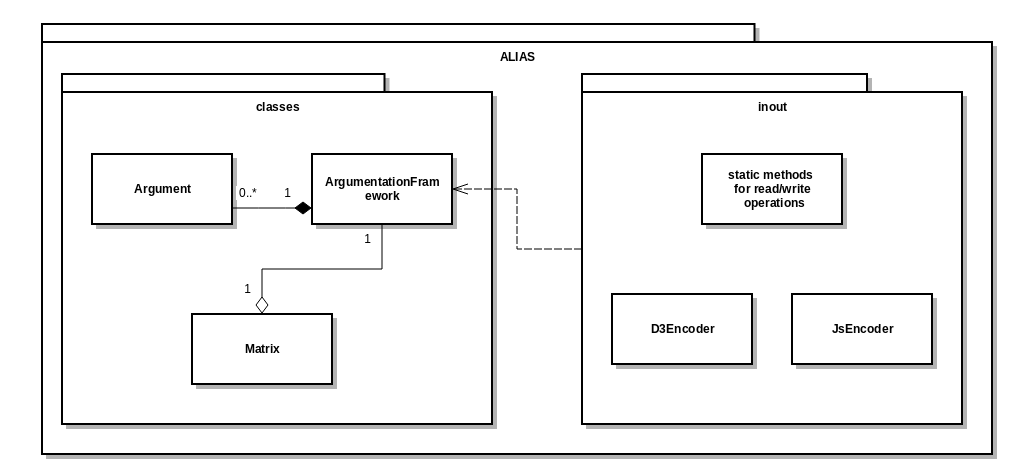
\includegraphics[width=\textwidth]{aliasv2_uml}
	\caption{ALIAS New Design - UML diagram}
	\label{fig:aliasUml2}
\end{figure}

\begin{figure}[h]
	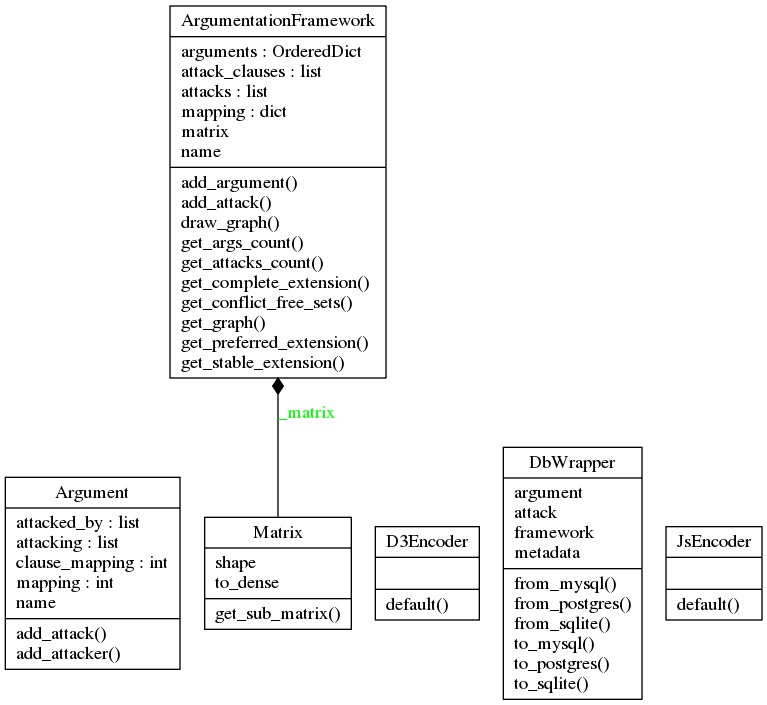
\includegraphics[width=\textwidth]{aliasv2_class}
	\caption{ALIAS New Design - class diagram}
	\label{fig:aliasUml2}
\end{figure}

\subsection{Web User Interface Design}
The Web Interface will consist of a single page, with menu options at the top of the page and computed solutions displayed at the side of the page in form of the list. The graph representation of the argumentation framework will be displayed centrally taking up the remaining space. This way, the real estate of the web page will be used most efficiently by concentrating on the graph structure. 

\subsubsection{Usability}
The design of User Interface should be done with usability in mind. Following usability criteria will be addressed during design and implementation stages:
\begin{itemize}
	\item Number of pages - website will consist of a single page, where the requests to ALIAS will be made through ajax calls
	\item Easy to follow layout - website will consist of three main elements: toolbar, list of possible solutions and graph area. Furthermore, graph area will take majority of the space
	\item Clear functionality - the available functionality will be clear to user as all the buttons and navigation links will be clearly labeled and additional information provided in the modal windows
	\item Feedback - website should provide feedback to user, especially when certain operations take long time to complete
\end{itemize}

\subsubsection{RESTful Design}
RESTful API will be implemented in order to allow user to interact with ALIAS application through web interface. The web extension will be divided into 2 tiers: front-end and back-end. 

Front-end will be implemented using HTML5 with Bootstrap framework and cytoscape.js \citep{cytoscapejs} for rendering argumentation frameworks as graphs. Furthermoe, JQuery will be used on the client side in order to send request to web server.

Back-end will be implemented using Python Flask \citep{flaskDocs} micro-framework.

\paragraph{Exposed API Routes} 
In order for the user to interact with ALIAS through web interface, certain methods and behaviours of ALIAS will have to be exposed through API routes. The list of required routes is shown in table \ref{table:apiRoutes}. Those represents the main functionality of ALIAS, where user can create new Argumentation Framework, add arguments and attacks, or load and parse tgf file.


\begin{table}[]
	\centering
		\begin{tabular}{|p{7cm}|p{1.5cm}|p{4.5cm}|}
			\hline
			\textbf{Route} & \textbf{Method} & \textbf{Operation}  \\ \hline \hline
			/ & GET & Gets home page \\ \hline
			/framework/\textless{}af\_id\textgreater{} & GET & Request for example framework, where \textless{}af\_id\textgreater is id of the framework \\ \hline
			/extension/\textless{}ext\_id\textgreater{} & GET & Request for extension to be calculated, where \textless{}ext\_id\textgreater is id of the extension \\ \hline
			/uploadFile & GET & Uploads and parses the tgf file into Argumentation Framework \\ \hline
			/addArgument/\textless{}arg\textgreater{} & GET & Request to add argument \textless{}arg\textgreater to current Argumentation Framework \\ \hline
			/addAttack/\textless{}attacker\textgreater{}/\textless{}attacked\textgreater{} & GET & Request to add attack from \textless{}attacker\textgreater to \textless{}attacked\textgreater to current Argumentation Framework \\ \hline
			/newFramework & GET & Request to create new Argumentation Framework \\ \hline
		\end{tabular}%
	\caption{ALIAS Web UI API Routes}
	\label{table:apiRoutes}
\end{table}

\subsection{Project Structure}
The structure of ALIAS will have to be changed in order to allow for the changes required for the new implementation. As mentioned previously the semantics module will be removed from alias package. Furthermore, any existing tests will be removed and replaced by Tests structure that will contain the tests of functionality of argumentationframework and short performance tests using predefined frameworks.

Furthermore, web\_interface folder will be added to store artifacts required for ALIAS web interface extension. It will consist of static folder, which in turn will contain css and js files in their corresponding locations, folder for storing uploaded files, Flask config file and app.py, which contains logic for API routing.

\begin{figure}[!ht]
	\dirtree{%
	.1 /.
	.2 alias.
	.3 classes.
	.4 argument.py.
	.4 argumentationframework.py.
	.4 matrix.py.
	.3 inout.
	.4 apx.py.
	.4 d3\_js.py.
	.4 dot.py.
	.4 js.py.
	.4 netx.py.
	.4 plot.py.
	.4 tgf.py.
	.2 Tests.
	.3 frameworks.
	.4 ...
	.3 argumentationFrameworkTests.py.
	.3 performanceTests.py.
	.3 testHelper.py.
	.2 web\_interface.
	.3 static.
	.4 css.
	.5 main.css.
	.4 js.
	.5 main.js.
	.3 templates.
	.4 index.html.
	.3 upload.
	.3 app.py.
	.3 config.py.
	}
	\caption{Proposed Project Structure}
	\label{fig:structureTree}
\end{figure}